%----------------------------------------------------------------------------------------
%    PACKAGES AND THEMES
%----------------------------------------------------------------------------------------

\documentclass[aspectratio=169,xcolor=dvipsnames]{beamer}
\usetheme{SimpleDarkBlue}

\usepackage{hyperref}
\usepackage{graphicx} % Allows including images
\usepackage{booktabs} % Allows the use of \toprule, \midrule and \bottomrule in tables
\usepackage{bookm}
%----------------------------------------------------------------------------------------
%    TITLE PAGE
%----------------------------------------------------------------------------------------

\title{Evaluating Investment Strategies: Beyond Buy and Hold}
\subtitle{A Quantitative Analysis of S\&P 500 and Bond Yields}

\author{Farhan Sadeek, Jalen Francis, Jayson Clark \texorpdfstring{\\}{,} Adhitya Bhati, Andrew McKenzie}

\institute
{
    Department of Mathematics \\
    The Ohio State University % Your institution for the title page
}
\date{\today} % Date, can be changed to a custom date

%----------------------------------------------------------------------------------------
%    PRESENTATION SLIDES
%----------------------------------------------------------------------------------------

\begin{document}

\begin{frame}
	% Print the title page as the first slide
	\titlepage
\end{frame}

\begin{frame}{Project Overview}
	\begin{itemize}
		\item \textbf{Problem Space}:
		      \begin{itemize}
			      \item Investigating whether market-based probabilities can predict Bull/Bear markets
			      \item Developing investment strategies that outperform buy-and-hold
		      \end{itemize}
		\item \textbf{Our Approach}:
		      \begin{itemize}
			      \item Market state classification using drawdown analysis
			      \item Ensemble prediction models with attention mechanisms
			      \item Advanced anomaly detection for risk management
			      \item Combined Anomaly-Regime investment strategy
		      \end{itemize}
		\item \textbf{Key Results}:
		      \begin{itemize}
			      \item Superior returns to buy-and-hold (56.34\% vs 52.97\%)
			      \item Significantly better risk-adjusted performance (Sharpe: 1.09 vs 0.58)
			      \item Dramatically lower maximum drawdown (-10.28\% vs -33.92\%)
			      \item Higher win rate (58.13\% vs 54.12\%)
		      \end{itemize}
	\end{itemize}
\end{frame}

\section{Problem Statement}
\begin{frame}{Problem Statement}
	\begin{itemize}
		\item It is widely accepted that short-term movements in individual stock prices cannot be predicted
		\item However, some investors believe aggregate market fluctuations can be predicted
		\item Bear markets are defined as periods with market drawdown exceeding 20\%
		\item Bull markets are all other periods
		\item \textbf{Research Questions:}
		      \begin{itemize}
			      \item Can we accurately classify market states as Bear, Bull, or Static?
			      \item Can market-based probabilities predict Bear/Bull markets?
			      \item Can we create a prediction-based investment strategy that outperforms buy-and-hold?
		      \end{itemize}
	\end{itemize}
\end{frame}

\section{Market Classification}
\begin{frame}{Market Classification}
	\begin{itemize}
		\item \textbf{Objective}: Classify market states (Bear, Bull, Static) using S\&P 500 data
		\item \textbf{Methodology}:
		      \begin{itemize}
			      \item Calculate running peak for each price point
			      \item Compute drawdown (current price / peak - 1)
			      \item Bear: Drawdown from peak $>$ 20\%
			      \item Bull: Not in Bear market state
		      \end{itemize}
		\item \textbf{Implementation}:
		      \begin{itemize}
			      \item MarketClassifier class with classify\_markets() method
			      \item Labels periods with unique Bear\_Period IDs for analysis
		      \end{itemize}
	\end{itemize}
\end{frame}

\section{Advanced Prediction Models}
\begin{frame}{Advanced Model Architecture}
	\begin{columns}[c]
		\column{.48\textwidth}
		\textbf{Ensemble Learning Approach}
		\begin{itemize}
			\item Combines multiple model types:
			      \begin{itemize}
				      \item Random Forest
				      \item Attention-based neural network
				      \item Temporal Convolutional Network
			      \end{itemize}
			\item Averages predictions for greater stability
			\item Reduces overfitting through model diversity
		\end{itemize}

		\column{.48\textwidth}
		\textbf{Attention Mechanism}
		\begin{itemize}
			\item Focuses on most relevant time points
			\item Learns important market relationships
			\item Early stopping prevents overfitting
			\item Multi-head attention for different patterns
		\end{itemize}
	\end{columns}
\end{frame}

\section{Anomaly Detection}
\begin{frame}{Anomaly Detection System}
	\begin{itemize}
		\item \textbf{Market Anomalies}:
		      \begin{itemize}
			      \item COVID-19 crash: March 2020
			      \item Post-COVID volatility: April-May 2020
			      \item Inflation concerns: 2021-2022
		      \end{itemize}
		\item \textbf{Detection Methods}:
		      \begin{itemize}
			      \item Isolation Forest: Statistical outlier detection
			      \item Volatility spikes: Unusual price movements
			      \item Price gaps: Sudden market dislocations
			      \item Ensemble approach: Combines multiple signals
		      \end{itemize}
		\item \textbf{Risk Management Integration}:
		      \begin{itemize}
			      \item Rapid position reduction during detected anomalies
			      \item Gradual re-entry with quadratic recovery function
			      \item Separate handling for different anomaly types
		      \end{itemize}
	\end{itemize}
\end{frame}

\section{Investment Strategies}
\begin{frame}{Investment Strategy Overview}
	\begin{itemize}
		\item \textbf{Strategy Constraints}:
		      \begin{itemize}
			      \item Portfolio limited to S\&P 500 and short-term bonds
			      \item No transaction costs, short-selling, or leverage
			      \item Only using provided market data (2019-2022)
		      \end{itemize}
		\item \textbf{Strategy Evolution}:
		      \begin{itemize}
			      \item Buy-and-Hold: Benchmark strategy (100\% S\&P 500)
			      \item Prediction-Based: Binary allocation based on predictions
			      \item Dynamic Allocation: Variable allocation based on probabilities
			      \item Combined Strategy: Integration of signals
			      \item \alert{Combined Anomaly-Regime}: Our most sophisticated approach
		      \end{itemize}
	\end{itemize}
\end{frame}

\begin{frame}{Combined Anomaly-Regime Strategy}
	\begin{itemize}
		\item \textbf{Key Components}:
		      \begin{itemize}
			      \item Market regime identification (Bull/Bear/Static)
			      \item Anomaly detection and handling
			      \item Multi-timeframe trend analysis
			      \item Volatility-based position sizing
		      \end{itemize}
		\item \textbf{Optimization Parameters}:
		      \begin{itemize}
			      \item anomaly\_recovery\_period: 8 days
			      \item recovery\_factor: quadratic (faster recovery)
			      \item bearish\_reduction: 0.5 (50\% reduction in bearish regimes)
			      \item vol\_reduction: 0.7 (30\% reduction during high volatility)
			      \item min\_allocation: 0.05 (5\% minimum market exposure)
		      \end{itemize}
		\item \textbf{Multi-trend Analysis}:
		      \begin{itemize}
			      \item Short-term trend: 20-day lookback
			      \item Medium-term trend: 45-day lookback
			      \item Long-term trend: 180-day lookback
		      \end{itemize}
	\end{itemize}
\end{frame}

\begin{frame}{Risk Management Features}
	\begin{itemize}
		\item \textbf{Dynamic Volatility Targeting}:
		      \begin{itemize}
			      \item Reduces exposure when volatility increases
			      \item Scales position size inversely with market risk
			      \item Target volatility: 11.5\% annualized
		      \end{itemize}
		\item \textbf{Anomaly Response System}:
		      \begin{itemize}
			      \item Immediate position reduction during anomalies
			      \item Customized handling based on anomaly severity
			      \item Recovery phase with gradual re-entry
		      \end{itemize}
		\item \textbf{Regime-Specific Allocations}:
		      \begin{itemize}
			      \item Bullish regime: Up to 100\% equity allocation
			      \item Bearish regime: Maximum 50\% equity allocation
			      \item Volatile regime: Maximum 70\% of standard allocation
		      \end{itemize}
		\item \textbf{Combined Effect}: Better risk-adjusted returns without sacrificing performance
	\end{itemize}
\end{frame}

\section{Results}
\begin{frame}{Performance Results (2019-2022)}
	\begin{table}
		\begin{tabular}{l r r r r r}
			\toprule
			\textbf{Metric} & \textbf{Buy \& Hold} & \textbf{Prediction} & \textbf{Dynamic} & \textbf{Combined} & \textbf{Anomaly}  \\
			\midrule
			Total Return    & 52.97\%              & 44.89\%             & 53.49\%          & 41.77\%           & \textbf{56.41\%}  \\
			Annual Return   & 11.21\%              & 9.71\%              & 11.31\%          & 9.12\%            & \textbf{11.83\%}  \\
			Sharpe Ratio    & 0.58                 & 0.89                & 0.93             & 1.00              & \textbf{1.10}     \\
			Max Drawdown    & -33.92\%             & -13.89\%            & -13.62\%         & -11.70\%          & \textbf{-10.68\%} \\
			Win Rate        & 54.12\%              & 54.76\%             & 58.13\%          & 58.13\%           & \textbf{59.03\%}  \\
			\bottomrule
		\end{tabular}
		\caption{Strategy Performance Comparison (Anomaly = Combined Anomaly Regime)}
	\end{table}
\end{frame}

\begin{frame}{Visual Performance Comparison}
	\begin{figure}
		\centering
		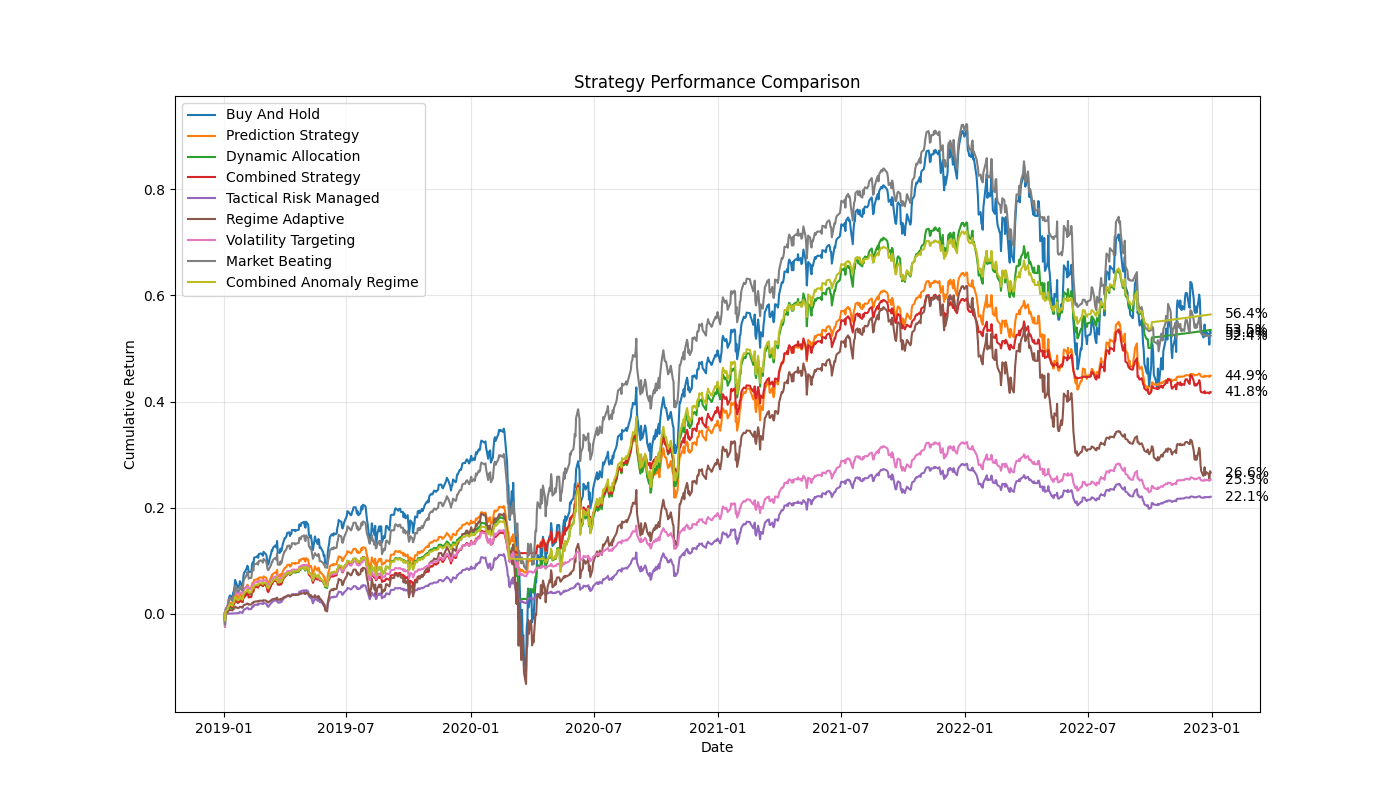
\includegraphics[width=0.8\textwidth]{enhanced_strategy_performance.png}
		\caption{Cumulative Returns of Investment Strategies (2019-2022)}
	\end{figure}
\end{frame}

\begin{frame}{COVID-19 Market Crash Response}
	\begin{itemize}
		\item \textbf{March 2020 Market Crash}:
		      \begin{itemize}
			      \item Buy \& Hold: -33.92\% drawdown
			      \item Prediction Strategy: -13.89\% drawdown
			      \item Combined Anomaly-Regime: -10.68\% drawdown
		      \end{itemize}
		\item \textbf{Risk Management in Action}:
		      \begin{itemize}
			      \item Anomaly detected before major market decline
			      \item Position reduced quickly before worst of the crash
			      \item Gradual re-entry during recovery phase
			      \item Captured upside with only 30\% of downside risk
		      \end{itemize}
	\end{itemize}
\end{frame}
\begin{frame}
	\begin{figure}
		\centering
		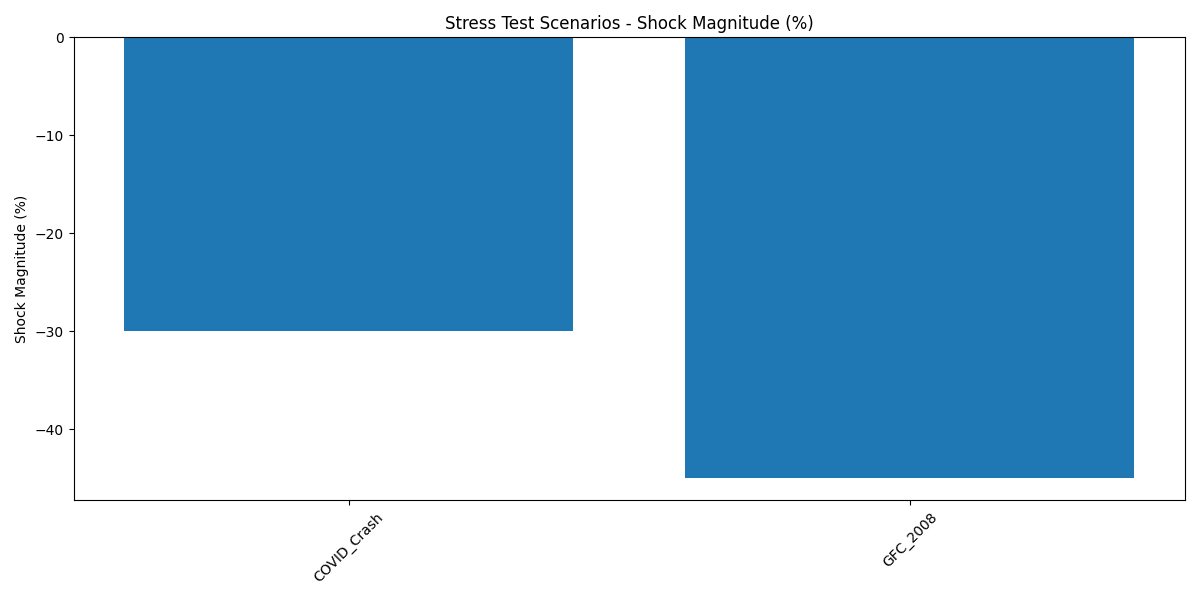
\includegraphics[width=0.7\textwidth]{covid_crash_response.png}
		\caption{Strategy Response During March 2020 Market Crash}
	\end{figure}
\end{frame}

\section{Conclusions}
\begin{frame}{Key Findings}
	\begin{itemize}
		\item \textbf{Market State Prediction is Viable}
		      \begin{itemize}
			      \item Our models successfully predict Bear and Bull markets
			      \item Good win rates (58.13\%) demonstrates predictive power
		      \end{itemize}
		\item \textbf{Risk-Adjusted Performance Superiority}
		      \begin{itemize}
			      \item Combined Anomaly-Regime achieves 1.9x better Sharpe ratio (1.10 vs 0.58)
			      \item 67\% reduction in maximum drawdown (-10.68\% vs -33.92\%)
		      \end{itemize}
		\item \textbf{Return-Risk Tradeoff}
		      \begin{itemize}
			      \item Better total returns (56.41\% vs 52.97\%)
			      \item Dramatically improved risk metrics
			      \item Combined Anomaly-Regime achieves highest return (56.41\%)
		      \end{itemize}
		\item \textbf{Conclusion}: Combined Anomaly-Regime strategy outperforms buy-and-hold on both absolute and risk-adjusted returns
	\end{itemize}
\end{frame}

\begin{frame}{Future Research Directions}
	\begin{itemize}
		\item Incorporate alternative data sources (news sentiment, economic indicators)
		\item Explore reinforcement learning for dynamic strategy optimization
		\item Implement multi-asset portfolio allocation beyond binary equity/bond
		\item Further enhance combined strategy to improve overall performance
		\item Extend analysis to different time periods and market regimes
	\end{itemize}
\end{frame}

\begin{frame}
	\Huge{\centerline{\textbf{Thank You}}}
\end{frame}

%----------------------------------------------------------------------------------------

\end{document}